\section{Durchführung}
\label{sec:Durchführung}

Mit der in \autoref{fig:messzeitkonst} dargestellten Schaltung wird zunächst die Zeitkonstante des RC-Kreises bestimmt.
Dazu wird eine gegen $τ$ kleine Frequenz $ω$ eingestellt, die so gewählt wird, dass sich $U_C(t)$ im Aufzeichnungsintervall um den Faktor 5 bis 10 ändert.
Ist eine geeignete Kurve sichtbar, werden Wertepaare $(U_C(t),t)$ im Abstand von $1 \,\unit{\milli\second}$ aufgenommen. \\

\begin{figure}
    \centering
    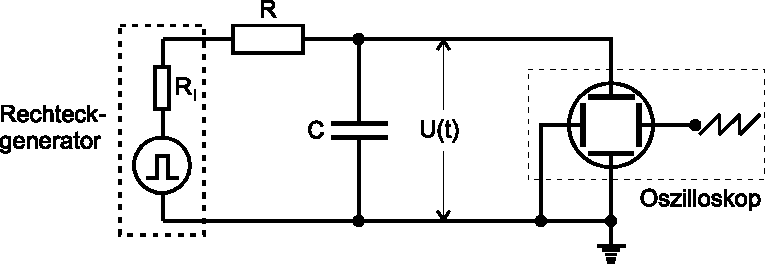
\includegraphics{figures/Messung a) Schaltung.pdf}
    \caption{Schaltung zur Bestimmung der Zeitkonstanten über die Auf- und Entladung des Kondensators\cite{ap08}.}
    \label{fig:messzeitkonst}
\end{figure}

Anschließend wird mit der in \autoref{fig:ampphase} aufgetragenen Schaltung die Frequenzabhängigkeit des RC-Kreises untersucht.

\begin{figure}
    \centering
    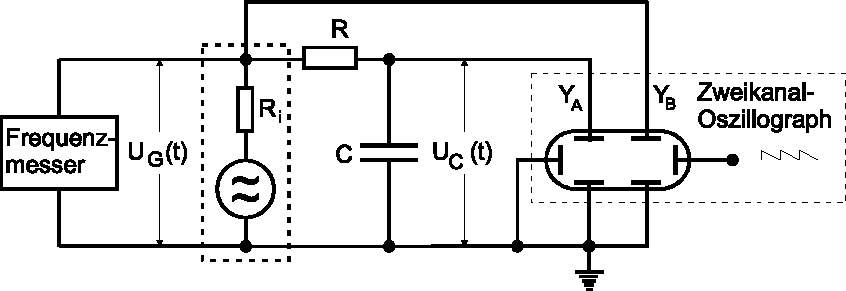
\includegraphics{figures/Messung b )& c).pdf}
    \caption{Schaltung zur Messung der Amplitude und Phasenverschiebung\cite{ap08}.}
    \label{fig:ampphase}
\end{figure}
Die Generatorspannung und die Kondensatorspannung werden dabei auf die beiden unterschiedlichen Eingänge des Oszilloskop gelegt.
Es werden die Amplitude und die Phasenverschiebung gemessen.

